\documentclass{article}

\usepackage{listings}
\lstset{
basicstyle=\small\ttfamily,
columns=flexible,
breaklines=true
}


\usepackage[T1]{fontenc}
\usepackage[utf8]{inputenc}
\usepackage{lmodern}
\usepackage{amsmath}
\usepackage{graphicx}
\usepackage{bm}
\usepackage{fancyvrb}

\author{Sigrid Videm}
\title{Project 5}

\begin{document}
\maketitle

\section{Abstract} 
I have implemented three schemes for solving the one dimensional diffusion equation numerically, and I have compared the results to the analytical solution of the problem. With a spatial step length of $1/100$ there was not much difference to be found by visual inspection. I calculated the relative errors, and I found that making the spatial step length smaller improved the quality of the solution, but reducing the length of the time steps did not. The strange behaviour of the error has bothered me a lot, but I have not found the reason for it. The error was the same for all three schemes, but I have seen that the explicit scheme has a strong stability requirement. 

For the two dimensional diffusion equation I used the explicit scheme. I found a two dimensional problem which was easy to solve analytically, and used it to compare the numererical solution to the analytical one. Then I used the solver to solve a more complicated problem. The explicit scheme for the two dimensional problem seemed to have an even stronger stability requirement than the one dimensional one. 
\tableofcontents % for a table of contents


\section{Introduction}
In this project I have used finite differences to approximate the derivatives to develop three different schemes for solving the diffusion equation.
\begin{equation}\label{eqn:1}
 \frac{\partial^2 u(x,t)}{\partial x^2} =\frac{\partial u(x,t)}{\partial t}
\end{equation}
 I have used scaled variables - there are no pyhsical constants in my equation. Because of this, the solvers presented here, are suitable to solve any problem which can be modelled by equation \ref{eqn:1}. Examples are heat conduction problems and particle diffusion, but also the Schrödinger equation of a free particle is on the same form. Boundaries and initial conditions are presented in section 3.1, and in 3.1.1 is the analytical solution to the problem. The three schemes I'm going to use are The explicit scheme (section 3.1.2) which is easy to implement, but has a tedious stability requirement; the Implicit scheme (section 3.1.3) which needs to be solved as a matrix equation; and the Crank--Nicolson (section 3.1.4) scheme which is a combination of the two other schemes. Plots of the solutions and a discussion of the truncation error are in section 4.1.
 
I have found an analytical solution of the two dimensional diffusion equation, the solution is presented in section 3.2.1, and I have used the explicit scheme to solve it numerically. The explicit scheme is described in section 3.2.2, and the results are presented in section 4.2.
My code is available at \texttt{https://github.com/sigrivi/Project5}
\section{Methods}
\subsection{The 1D diffusion equation}
I want to solve the diffusion equation:
\begin{equation*}
 \frac{\partial^2 u(x,t)}{\partial x^2} =\frac{\partial u(x,t)}{\partial t}\hspace{0.5cm} t> 0 \hspace{0.5cm} x\in [0,L]
\end{equation*}
or
\begin{equation*}
u_{xx} = u_t,
\end{equation*}
with initial conditions

\begin{equation*}
u(x,0)= 0 \hspace{0.5cm} 0 < x < L
\end{equation*}
with $L=1$ the length of the $x$-region of interest. The 
boundary conditions are

\begin{equation*}
u(0,t)= 0 \hspace{0.5cm} t \ge 0,
\end{equation*}
and
\begin{equation*}
u(L,t)= 1 \hspace{0.5cm} t \ge 0.
\end{equation*}

To do this, I am going to use three different schemes: The explicit scheme, The implicit scheme and the Crank-Nicolson scheme. 
\subsubsection{The analytical solution}
With the boundaries $u(0,t) = 0$ and $u(L,t)= 1$, the system will reach a steady state as $t \rightarrow \infty $. The steady state function $v(x)$ must be a linear function, and satisfy the boundary conditions: 
\begin{equation*}
v(x) = \frac{x}{L}
\end{equation*}
The solution $u(x,t)$ can now be expressed as:
\begin{equation*}
u(x,t) = v(x) + w(x,t)
\end{equation*}
$w(x,t)$ is also a solution of $u_t = u_{xx}$, but with different boundaries. The boundaries are:
\begin{equation*}
w(0,t) = u(0,t)-v(0)= 0 - 0 = 0
\end{equation*}

\begin{equation*}
w(L,t) = u(L,t)-v(0)= 1 - 1 = 0
\end{equation*}
The initial condition is 
\begin{equation*}
w(x,0) = u(x,0)-v(x)= 0 - v(x) = -\frac{x}{L} \hspace{0.5cm} 0<x<L
\end{equation*}
To solve this system, I use the separation of variables technique. 
\begin{equation*}
w(x,t) = X(x)T(t)
\end{equation*}

$$w_t = T'X$$
$$w_{xx} = TX''$$
Inserted into the equation $w_t=w_{xx}$
$$TX''=T'X \implies \frac{T'}{T} = \frac{X''}{X} =\mathsf{ constant}$$
Let the constant be $-\lambda ^2$. We then have two separate equations:
\begin{equation*}
T' + \lambda^2 T = 0 \implies T=e^{-\lambda^2 t}
\end{equation*}

\begin{equation*}
X'' + \lambda^2X = 0 \implies X=A \sin \lambda x + B\cos \lambda x
\end{equation*}
The boundary condition $w(0,t) = 0$ requires $B=0$, while the boundary condition $w(L,t)=1$ requires that $\lambda$ is a multiple of $\pi$: $\lambda_k = k\pi /L$, where $k = 1,2,3,...$. 
We now have the solution $w(x,t)=X(x)T(t)$
\begin{equation*}
w(x,t) = \sum_k A_k \sin \frac{k \pi x}{L}\cdot e^{-k^2\pi^2 t /L^2}
\end{equation*}

I can find the coefficients $A_k$ by using the initial condition $w(x,0)=-x/L$
\begin{equation*}
w(x,0) = \sum_k A_k \sin \frac{k \pi x}{L}= \frac{-x}{L}
\end{equation*}
$A_k$ are the Fourier coefficients (page 19 in the lecture notes \cite{PDE})
\begin{equation*}
A_k = \int_0^L\frac{-x}{L} \sin \frac{k \pi x}{L} dx = - \frac{2}{L}\bigg[\frac{1}{(k\pi)^2} \sin k \pi x - \frac{x}{k\pi}\cos k\pi x \bigg]_0^1 = \frac{2}{Lk\pi}\cos k\pi
\end{equation*}

The soulution $u(x,t) = w(x,t) + x/L$ of the original problem is 
\begin{equation}
u(x,t)=\sum_k \frac{2}{Lk\pi}\cos k\pi \cdot \sin \frac{k\pi x}{L} \cdot e^{-k^2\pi^2 t /L^2} + \frac{x}{L}
\end{equation}

In order to calculate this analytical solution, I made the function \texttt{exactsolution(x,t)}, which returns the solution \texttt{u} for a given time \texttt{t}. The vector \texttt{x} represents the $x$ values. It was surprisingly hard for me to solve this problem, and I had a lot of help from Boyce and DiPrima \cite{Boyce}.
\subsubsection{The explicit scheme}
The explicit scheme uses the Euler forward approximation for the time derivative:
\begin{equation*}
\frac{\partial u}{\partial t} = \frac{u_{j+1}-u_j}{\Delta t}+ O(\Delta t) \approx \frac{u_{j+1}-u_j}{\Delta t}
\end{equation*}
This approximation has an error of $O(\Delta t)$. For the second order spatial derivative, I use the central difference approximation:  
\begin{equation*}
\frac{\partial^2 u}{\partial^2 x} = \frac{u_{i+1}-2u_i + u_{i-1}}{(\Delta x)^2} + O((\Delta x)^2) \approx \frac{u_{i+1}-2u_i + u_{i-1}}{(\Delta x)^2}
\end{equation*}

Which has an error of $O((\Delta x)^2)$. The diffusion equation can now be approximated with:

\begin{equation*}
\frac{u_{i}^{l+1}-u_i^l}{\Delta t} \approx \frac{u_{i+1}^{l}-2u_i^{l} + u_{i-1}^l}{(\Delta x)^2}
\end{equation*}
\begin{equation}\label{eqn:3}
u_{i}^{l+1}= \frac{\Delta t}{(\Delta x)^2}(u_{i+1}^l-2u_{i}^l + u_{i-1}^{l})+u_{i}^{l}=\alpha(u_{i+1}^l-2u_{i}^l + u_{i-1}^{l})+u_{i}^{l}
\end{equation}

The truncation error of the explicit scheme is of $O((\Delta x)^2)$ and $O(\Delta t)$. Equation \ref{eqn:3} can be rewritten as a matrix--vector product.
\begin{equation*}
\bm{u}^{l+1}
=
\begin{bmatrix}
1-2\alpha & \alpha & 0 & 0 \\
\alpha & 1-2\alpha & \alpha & 0 \\
 &  & \ddots  &  \\
0 & 0 & \alpha & 1-2\alpha \\
\end{bmatrix}
\bm{u}^{l}
\end{equation*}
There is a danger of using the explicit scheme. In the lecture notes \cite{PDE}, the spectral radius of the matrix is used to show that the explicit scheme is stable only if $\Delta t / (\Delta x)^2 \leq 1/2$. The treacherousness of the explicit method is revealed in section 4.1.1. 

The function \texttt{explicitsolver(Nt,tfinal,Nx,frequency)} is an implementation of the explicit scheme. It does \texttt{Nt} steps, each step is made by calling the function \texttt{forwardstep}:
\begin{verbatim}
def forwardstep(u, alpha): 
    unew = u.copy()
    unew[0] = (1-2*alpha)*u[0] + alpha*(u[1]) 
    unew[1:Nx] = (1-2*alpha)*u[1:Nx] + alpha*(u[2:Nx+1]+u[0:Nx-1])
	
	return(unew)
\end{verbatim}
\texttt{forwardstep} returns the vector \texttt{unew}, which is the solution at the current time step. Every \texttt{Nt/frequency} solution is stored in a matrix \texttt{U}, which is returned from  \texttt{explicitsolver}. 
My implementation of the explicit scheme is in \texttt{project5c.py}.
\subsubsection{The implicit scheme}
For the implcit scheme, I use the same approximation for the spatial derivative, but the Euler backward approximation for the time derivative.

\begin{equation*}
\frac{\partial u}{\partial t} = \frac{u^l-u^{l-1}}{\Delta t}+ O(\Delta t) \approx \frac{u^l-u^{l-1}}{\Delta t}
\end{equation*}
The approximation to the diffusion equation is
\begin{equation*}
\frac{u_{i}^l-u_{i}^{l-1}}{\Delta t} \approx \frac{u_{i+1}^l-2u_i^l + u_{i-1}^l}{(\Delta x)^2}
\end{equation*}

with $\alpha = \Delta t/ (\Delta x)^2$:
\begin{equation*}
u_{i}^l(1+2\alpha) -\alpha u_{i+1}^l-\alpha u_{i-1}^l=u_i^{l-1}
\end{equation*}
Now, the new solution is no longer determined explicitely by the previous one. I find the solution by converting the problem into a matrix equation:
\begin{equation}
\begin{bmatrix}
1+2\alpha & -\alpha & 0 & 0 \\
-\alpha & 1+2\alpha & -\alpha & 0 \\
 &  & \ddots  &  \\
0 & 0 & -\alpha & 1+2\alpha \\
\end{bmatrix}
\bm{u}^l
=
\bm{u}^{l-1}
\end{equation}

To solve this equation, I use Gaussian elimination to get an upper triangular matrix, and backsubstitution to find the solution. I have explained the algorithm in more detail in project 1 \cite{Project1}. The functions \texttt{rowreduction} and \texttt{backsubstitution} does the job for me.

\begin{verbatim}
def rowreduction(A,u):
    for i in range(A.shape[0]-1): # Gaussian elimination
        coeff=A[i+1,i]/A[i,i]
        A[i+1,i+1]=A[i+1,i+1]-A[i,i+1]*coeff
        u[i+1]=u[i+1]-u[i]*coeff
\end{verbatim}

and 
\begin{verbatim}
def backsubstitution(A, u, alpha): 
    Nx = A.shape[0]
    solution = u.copy()
    solution[Nx] = 1                        # boundary condition
    for i in range(1,Nx+1):                 #backward substitution
        k = Nx-i
        solution[k] = (u[k]+alpha*solution[k+1])/A[k,k]
    return(solution)
\end{verbatim}
The matrix equation has to be solved for every time step. Therfore, the function  \texttt{implictsolver(Nt,tfinal,Nx,frequency)} loops over \texttt{Nt}, where \texttt{Nt} is the number of time steps. \texttt{implictsolver} constructs the matrix \texttt{A} and calls \texttt{rowreduction} and \texttt{backsubstitution} for every time step. Every \texttt{Nt/frequency} solution is stored in a matrix \texttt{U}, which is returned from  \texttt{implicitsolver}.
The implicit scheme has the same truncation errors as those of the explicit, because the approximations to the derivatives are of the same order, but it is shown in the lecture notes \cite{PDE} that this scheme is stable for all $\alpha$.

\subsubsection{Crank--Nicolson scheme}
For the Crank--Nicolson scheme, the approximations of the derivatives are:
\begin{equation*}
\frac{\partial u}{\partial t } \approx \frac{u_i^{l+1}-u_i^l}{\Delta t}
\end{equation*}

\begin{equation*}
\frac{\partial^2 u}{\partial x^2} \approx \frac{1}{2}(\frac{u_{i+1}^{l+1}-2u_i^{l+1}+u_{i-1}^{l+1}}{\Delta x^2}+ \frac{u_{i+1}^{l}-2u_i^{l}+u_{i-1}^{l}}{\Delta x^2})
\end{equation*}

with $\alpha =  \frac{\Delta t} {2(\Delta x)^2}$:

\begin{equation*}
u_i^{l+1}-u_i^l = \alpha(u_{i+1}^{l+1}-2u_i^{l+1}+u_{i-1}^{l+1} + u_{i+1}^{l}-2u_i^{l}+u_{i-1}^{l} )
\end{equation*}

reorganize so that all $u^{l+1}$ terms are on the left side:

\begin{equation*}
u_i^{l+1} - \alpha u_{i+1}^{l+1} + 2\alpha u_i^{l+1}- \alpha u_{i-1}^{l+1} = u_i^l+  \alpha u_{i+1}^{l}-2\alpha u_i^{l}+ \alpha u_{i-1}^{l} 
\end{equation*}

Rewrite as matrix vector products:

\begin{equation*}
\begin{bmatrix}
1+2\alpha & -\alpha & 0 & 0 \\
-\alpha & 1+2\alpha & -\alpha & 0 \\
 &  & \ddots  &  \\
0 & 0 & -\alpha & 1+2\alpha \\
\end{bmatrix}
\bm{u}^{l+1}
=
\begin{bmatrix}
1-2\alpha & \alpha & 0 & 0 \\
\alpha & 1-2\alpha & \alpha & 0 \\
 &  & \ddots  &  \\
0 & 0 & \alpha & 1-2\alpha \\
\end{bmatrix}
\bm{u}^{l}
\end{equation*}

The right hand side is identical to the matrix vector product of the explicit method, while the left hand side is identical to the matrix vector product of the implicit method. The only difference is $\alpha$.  That means that I can use the forward step function to calcuate the rigth hand side, and then use use row reduction and backsubstitution as I did in the implicit scheme. 

\begin{verbatim}
def cranknicolson(Nt,tfinal,Nx,frequency): 

    alpha,u,U,counter = initialize(Nt,tfinal,Nx,frequency)
    beta = alpha/2
    B = makeA(Nx,beta)

    for t in range(Nt):
        u = forwardstep(u, beta)

        A = B.copy()
        rowreduction(A, u)

        u = backsubstitution(A, u, beta)

        if t%frequency == 0: # to store every frequency solution
            U[1:,counter] = u
            counter += 1
    return(U)
\end{verbatim}

In the lecture notes, it is shown that the error of the Crank Nicolson scheme is $O(h^2)$ and $O(\Delta t)^2$, and that the Crank Nicolson scheme is stable for all $\alpha$
\subsection{The 2D diffusion equation}

In two dimensions, the diffusion equation look like this: 

\begin{equation*}
\frac{\partial u}{\partial t} = \frac{\partial^2 u}{\partial x^2}+\frac{\partial^2 u}{\partial y^2}
\end{equation*}

\subsubsection{An analytic solution}
I learned a lot of things from the 1 dimensional case. 1) Separation of variables is a good technique 2) the solution will be easier to find if the boundaries are zero and if 3) the initial condition is a sine function. When I am free to choose the boundaries as I like, I do it the simple way, and I will use $L=1$ as the length of the system in both x and y direction. The boundaries I choose are:

$$u(0,y,t)=u(1,y,t)=u(x,0,t)=u(x,1,t)=0$$
And the initial condition: $u(x,y,0) = \sin \pi x \sin \pi y$

I can write $u(x,y,t) = X(x) Y(y) T(t)$, and I find $T=e^{-\lambda^2 t}$ like i did in the 1D case. Nothing stops me from separating the variables again:
$$
\frac{X''}{X}= -\frac{Y''}{Y}-\lambda^2 = -\kappa^2
$$
This gives an equation for $X$ which is similar to the 1D

$$
X(x) = A_x \sin \kappa x + B_x \cos \kappa x
$$

The boundary conditions require $B_x = 0$, and $\kappa$ must be a muliple of $\pi$. The initial condition(which indeed was wisely choosen) gives $A_k =1$ and $\kappa = \pi$. For $Y$, we have
$$\frac{Y''}{Y}= \kappa^2 -\lambda^2 $$
With $ \kappa^2 -\lambda^2 = -\eta ^2$
$$Y = A_y \sin \eta y +B_y \cos \eta y$$
Again, boundary conditions require $B_y = 0$, and $\eta$ a multiple of $\pi$. Initial conditions give $A_y = 1$ $\eta = \pi$. When $\kappa$ and $\eta$ are determined, I can determine $\lambda^2= \eta^2+\kappa^2=2\pi ^2 $. The solution is
\begin{equation}
u(x,y,t) = e^{-2\pi^2 t}\sin \pi x \sin \pi y
\end{equation}
\subsubsection{The explicit scheme}
The explicit scheme for the 2 dimensional diffusion equation uses the Euler forward approximation for the time derivative, and the central difference approximation for the spatial derivative:
\begin{equation*}
\frac{u_{i,j}^{l+1}-u_{i,j}^l}{\Delta t} \approx \frac{u_{i+1,j}^{l}-2u_{i,j}^{l} + u_{i-1,j}^l}{(\Delta x)^2}+\frac{u_{i,j+1}^{l}-2u_{i,j}^{l} + u_{i,j-1}^l}{(\Delta y)^2}
\end{equation*}
With $\Delta x = \Delta y = h$, I can rewrite the equation so that i get $u_{i,j}^{l+1}$ alone on the left hand side:
\begin{equation*}
u_{i,j}^{l+1} = \alpha( u_{i+1,j}^{l} + u_{i-1,j}^l + u_{i,j+1}^{l} + u_{i,j-1}^l-4u_{i,j}^{l})+u_{i,j}^l
\end{equation*}
To solve this, I made the function \texttt{explicitsolver2D(Nt,tfinal,Nx,frequency,n)}. The \texttt{explicitsolver2D} makes a matrix \texttt{U} of size \texttt{NX+1} and the vector \texttt{axis} which concist of evenly distributed numbers between 0 and 1. The elements of \texttt{U} are 
\begin{verbatim}
	x0 = np.sin(axis *np.pi)
	np.outer(x0, x0, U)
\end{verbatim}

For every time step, the elements of \texttt{U} are used to update \texttt{U}:
\begin{verbatim}
for l in range(Nt):

    U[1:Nx,1:Nx] = alpha*(U[2:Nx+1,1:Nx] + U[0:Nx-1,1:Nx]
+ U[1:Nx,2:Nx+1] + U[1:Nx,0:Nx-1] - 4*U[1:Nx,1:Nx]) + U[1:Nx,1:Nx]
\end{verbatim}

The function returns one matrix, namely solution number \texttt{frequency * n}, but it can easily be modified so that it returns other solutions as well. I also included a plot function which plots a cross section for different times. A contour plot at $t=0.02$ and the cross section plot are in section 4.2.1. 
Because I cannot come up with a plausible physical system that is described by these boundary and initial conditions, I used the explicit solver to solve the equation for different conditions:
$$
u(0,y,t)=u(x,0,t)=0 \wedge
u(1,y,t) =u(x,1,t) =1 
$$$$
u(x,y,0) = 0 , 0<x<1, 0<y<1
$$
These conditions could describe a block being in contact with a heat reservoir at high temperature at tweo sides, and low temperature at the other two sides. The initial temperature of the block is the same a that of the low temperature reservoir.  Plots illustrating the evolving system are in section 4.2.3.
The code for the explicit scheme is in \texttt{project5f.py}
\section{Results and Discussion}
\subsection{The 1D diffusion equation}
\begin{figure}
  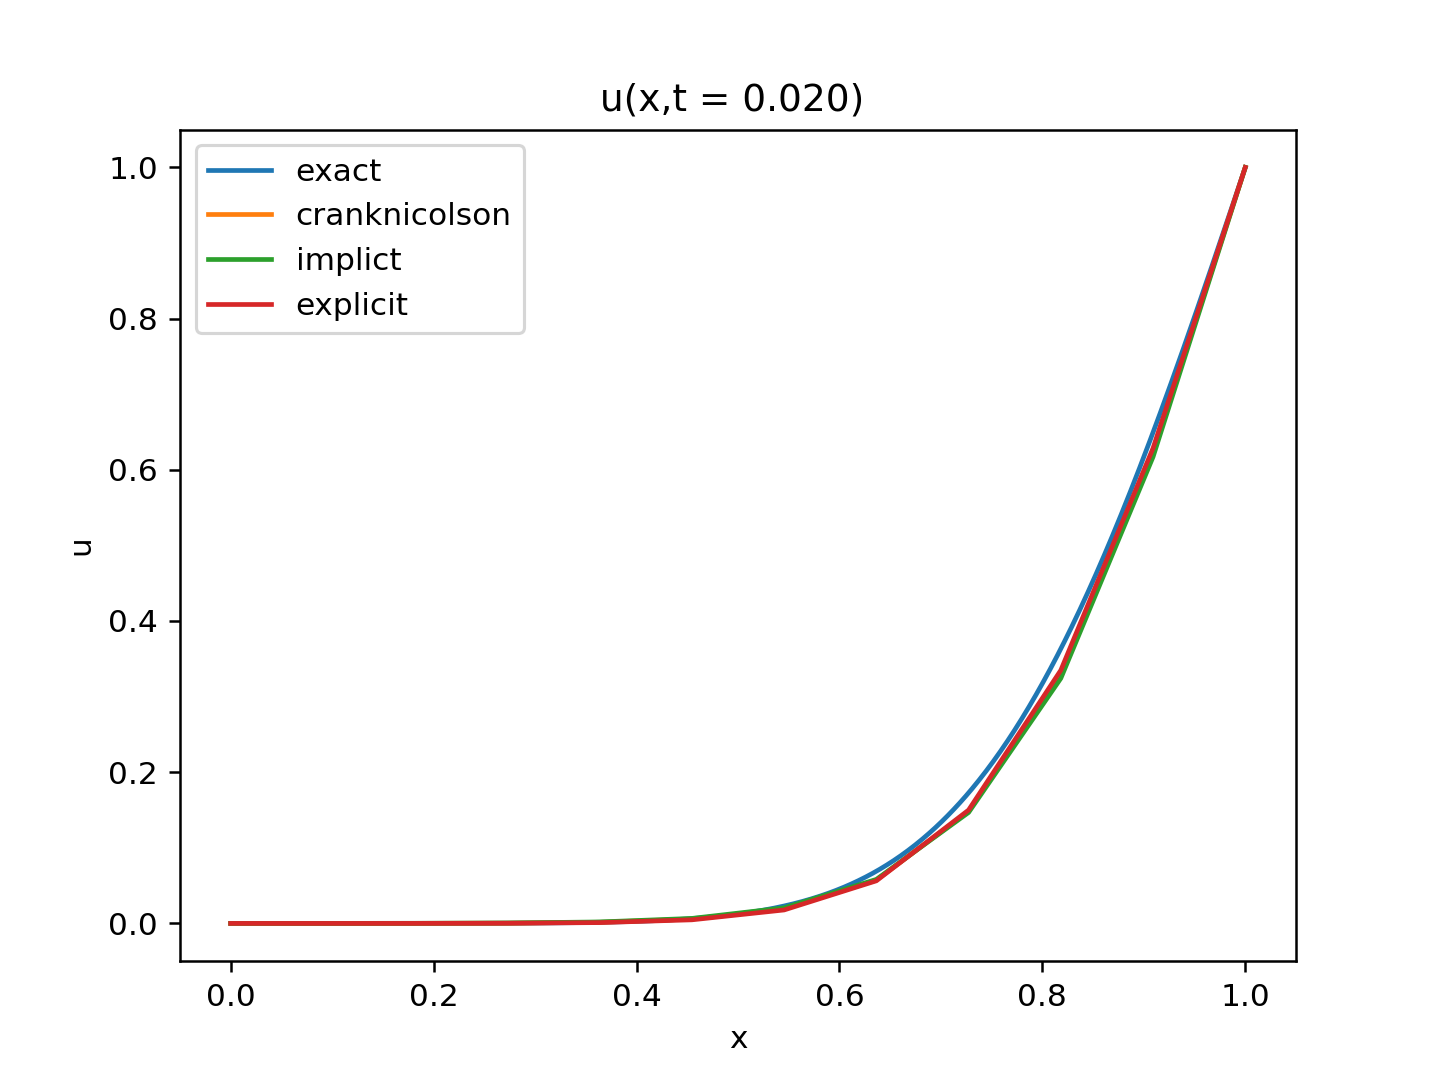
\includegraphics[width=\linewidth]{Nt1000Nx10t02.png}
  \caption{The exact solution plotted together with the numerical ones. Nx = 10, Nt = 1000. The numerical solutions lie close to each other, and below the exact one}
  \label{fig:Nt1000Nx10t02}
\end{figure} 

\begin{figure}
  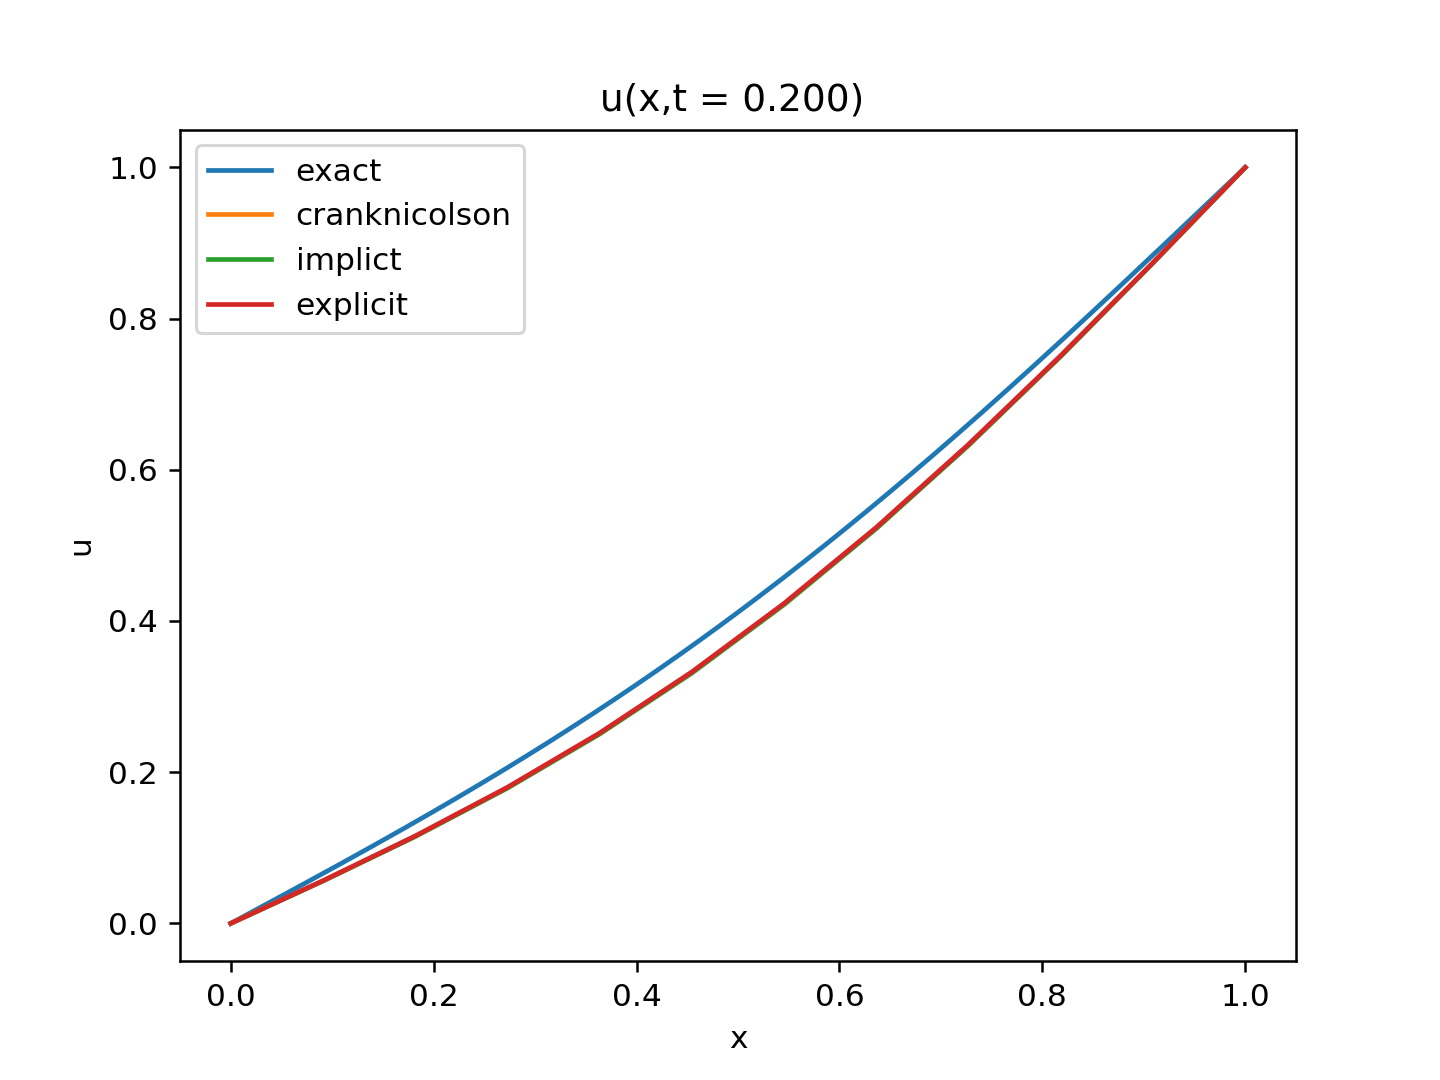
\includegraphics[width=\linewidth]{Nt1000Nx10t2.png}
  \caption{The exact solution plotted together with the nume)rical ones. Nx = 10, Nt = 1000.The numerical solutions are very similar, but differs from the exact one. }
  \label{fig:Nt1000Nx10t2}
\end{figure} 

\begin{figure}
  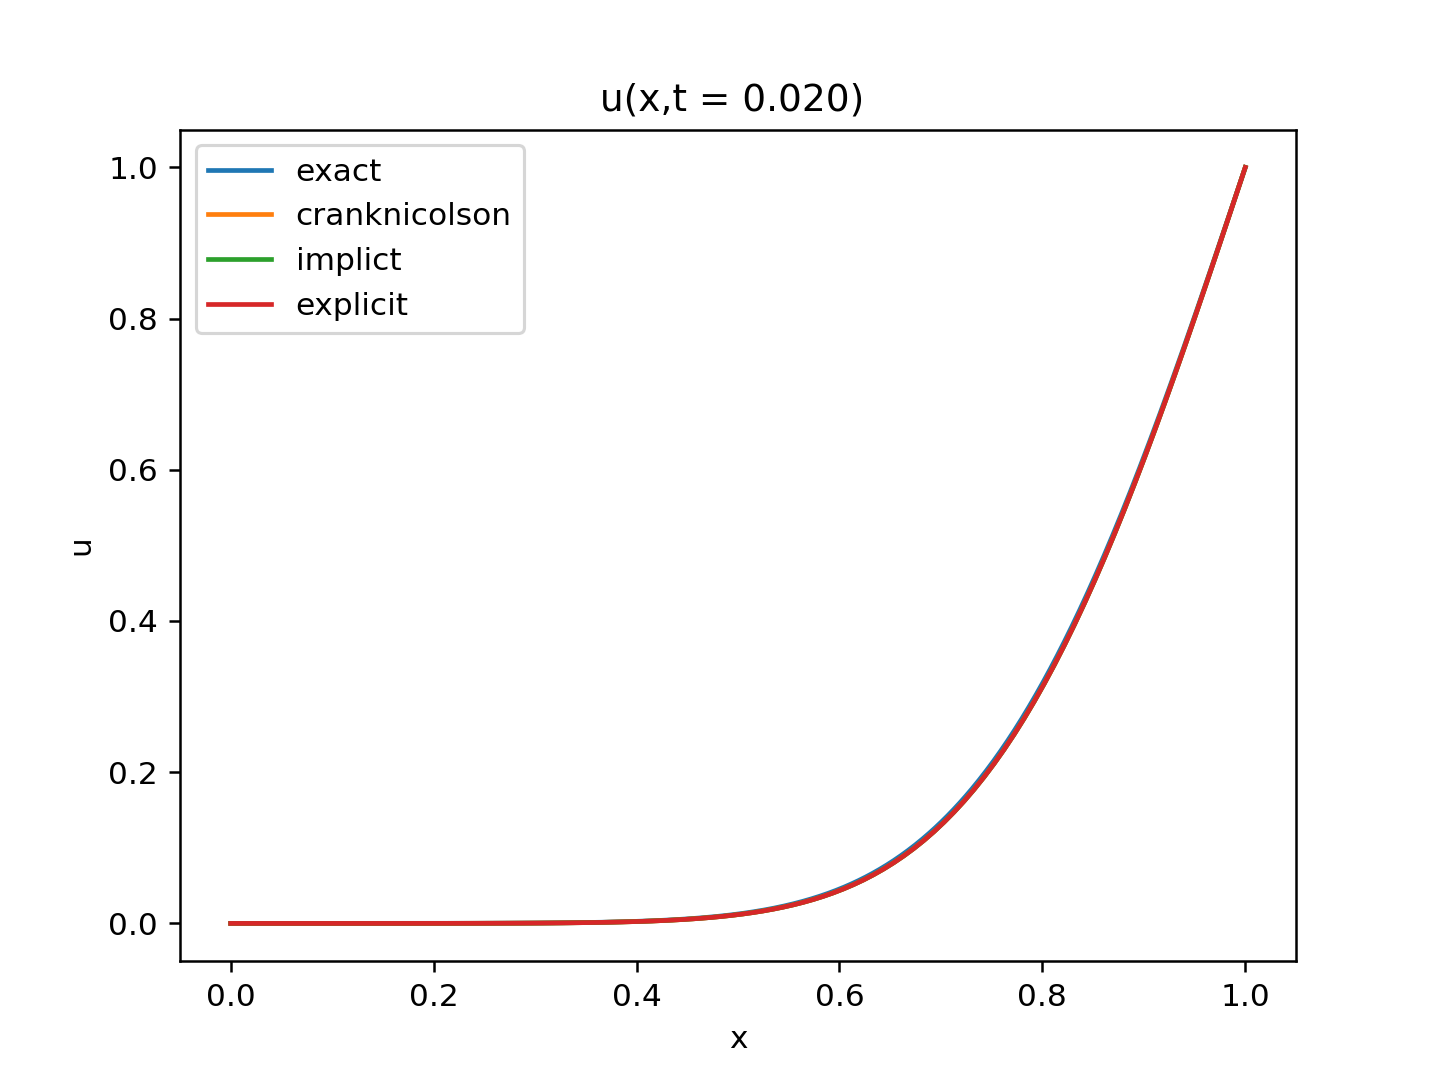
\includegraphics[width=\linewidth]{Nt100000Nx100t02.png}
  \caption{The exact solution plottet together with the numerical ones. Nx = 100, Nt = 100000. The solutions seems equal to the exact.}
  \label{fig:Nt100000Nx100t02}
\end{figure} 

\begin{figure}
  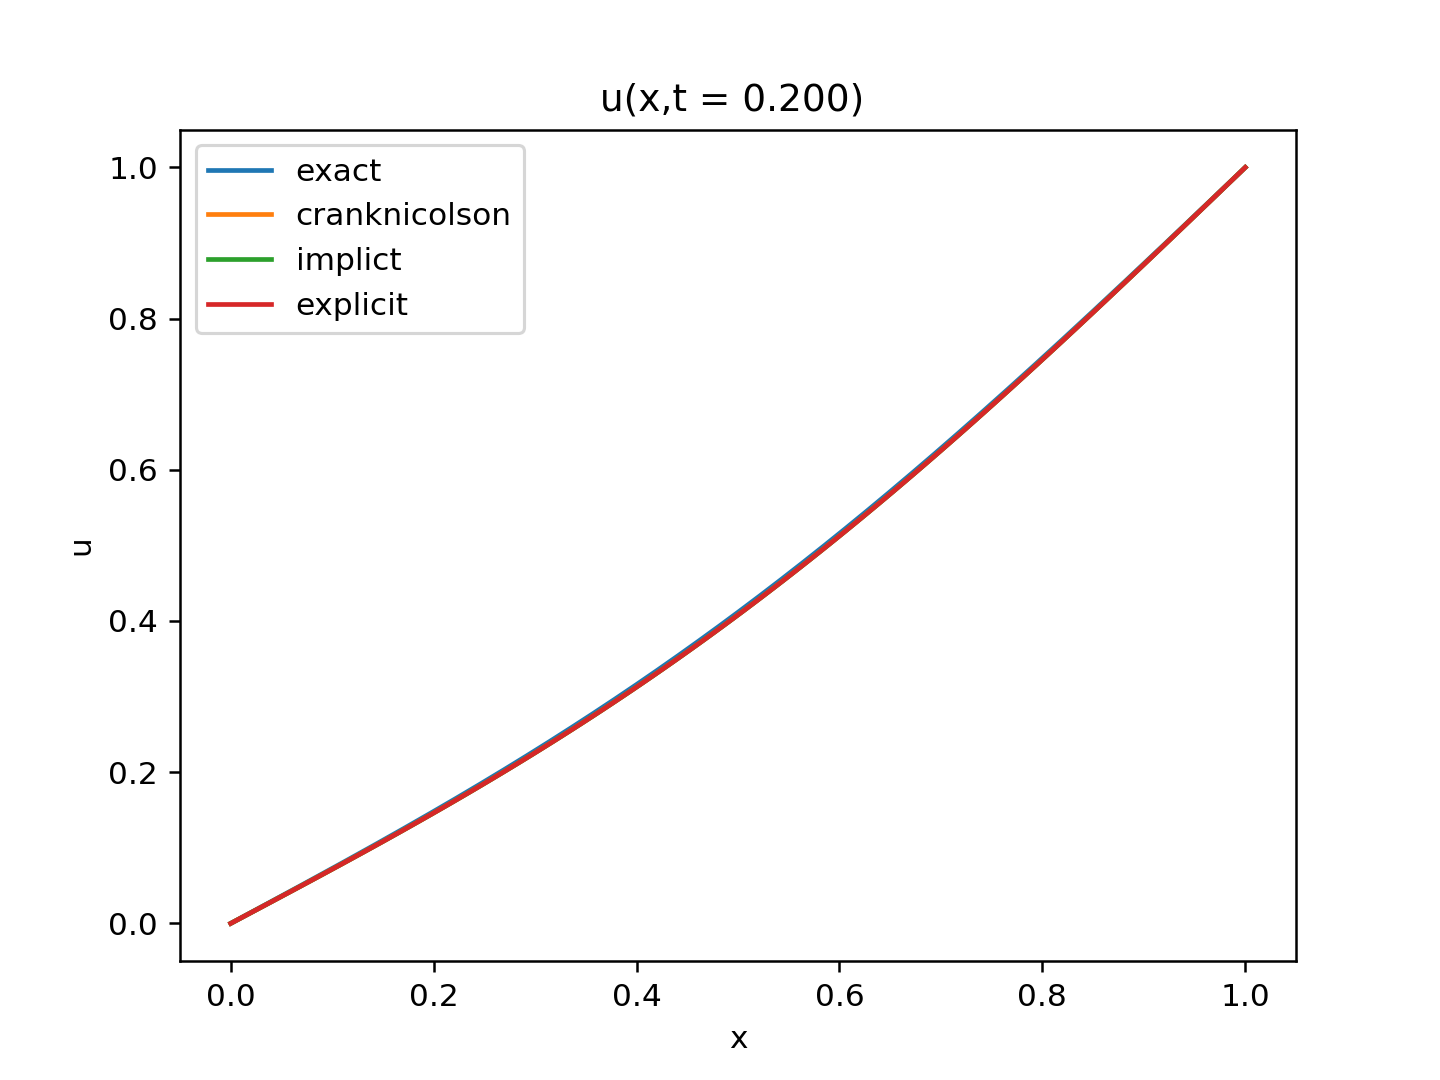
\includegraphics[width=\linewidth]{Nt100000Nx100t2.png}
  \caption{The exact solution plotted together with the numerical ones. Nx = 100, Nt = 100000. The solutions seems equal to the exact, and the graph is almost linear.}
  \label{fig:Nt100000Nx100t2}
\end{figure} 

The plots of figure \ref{fig:Nt1000Nx10t02}, \ref{fig:Nt1000Nx10t2}, \ref{fig:Nt100000Nx100t02} and \ref{fig:Nt100000Nx100t2} were made with the function \texttt{plotsolutions(ue,ui,uc, t}. Figure \ref{fig:Nt1000Nx10t02} shows the solutions from the three solvers together with the analytical solution at time $t=0.02$. $u$ is close to zero for a large part of the system, but the system has evolved from the discontinous initial state. The plot of figure \ref{fig:Nt1000Nx10t2} shows the same solution at $t=0.2$. At this time, the graphs are almost linear, the system is close to the stady state. For both plots, I used only 10 grid points for $x$. Still I got graphs that look similar to the exact one, but they all lie below the exact, and the difference is largerst in the middle. Then, I increased the number of grid point by a factor 10. The resulting plots are in figure \ref{fig:Nt100000Nx100t02} and \ref{fig:Nt100000Nx100t2}. Here it is difficult to distinguish the graphs by mere inspection. To look closer at the error, I calculated the error for varying $\Delta x $ ( table \ref{tab:table1}), and varying $\Delta t$ (table \ref{tab:table2}). 

\begin{table}[h!]
  \centering
  \caption{Relative error of the three schemes with varying $\Delta x$. $t=0.02$ and $\Delta t = 1/2000000$.}
  \label{tab:table1}
  \begin{tabular}{l||c|c|c}
    & $\Delta x = 1/10$ & $\Delta x = 1/100$ & $\Delta x = 1/1000$ \\
    \hline
    explicit & 0.0547113714079 & 0.00745993979441 & 0.000760541674696\\
    \hline
    implicit & 0.0547168789102 & 0.00746703401772  & 0.000767790391857\\
    \hline
    Cranck Nicolson & 0.0547141251303 & 0.00746348636423 & 0.000764152600736\\
  \end{tabular}
\end{table}

\begin{table}[h!]
  \centering
  \caption{Relative error of the three schemes with varying $\Delta $. $t=0.02$ and $\Delta x = 1/100$.}
  \label{tab:table2}
  \begin{tabular}{l||c|c|c}
    & $\Delta t = 1/20000$ & $\Delta t = 1/200000$ & $\Delta t = 1/2000000$ \\
    \hline
    explicit & 0.00620196835303 &  0.00734337585799 & 0.00745993979441\\
    \hline
    implicit & 0.0068930615448 & 0.00741431787145 & 0.00746703401772\\
    \hline
    Cranck Nicolson & 0.00653247845369 & 0.00737879226342 & 0.00746348636423\\
  \end{tabular}
\end{table}

Table \ref{tab:table1} shows how the relative error decreases with $\Delta x$. The error of the three schemes are of same magnitude, and the first leading digit is equal. According to the theory, decreasing $\Delta x$ should have the same effect on all three schemes. However, the error does not decrease as $(\Delta x)^2$. This indicates that there is someting wrong with either the way I calulate the error, or with the way I have implemented the schemes. The errors of table \ref{tab:table2} are even more disappointing. Increasing the number of time steps don't improve the error at all. What is more, the Crank Nicolson scheme is not doing better than the others. The latter leads me to think that there is something seriously wrong with how I have implemented the schemes, and that the big issue is the loop over \texttt{Nt} .
\subsubsection{The instability of the explicit scheme}

\begin{figure}
  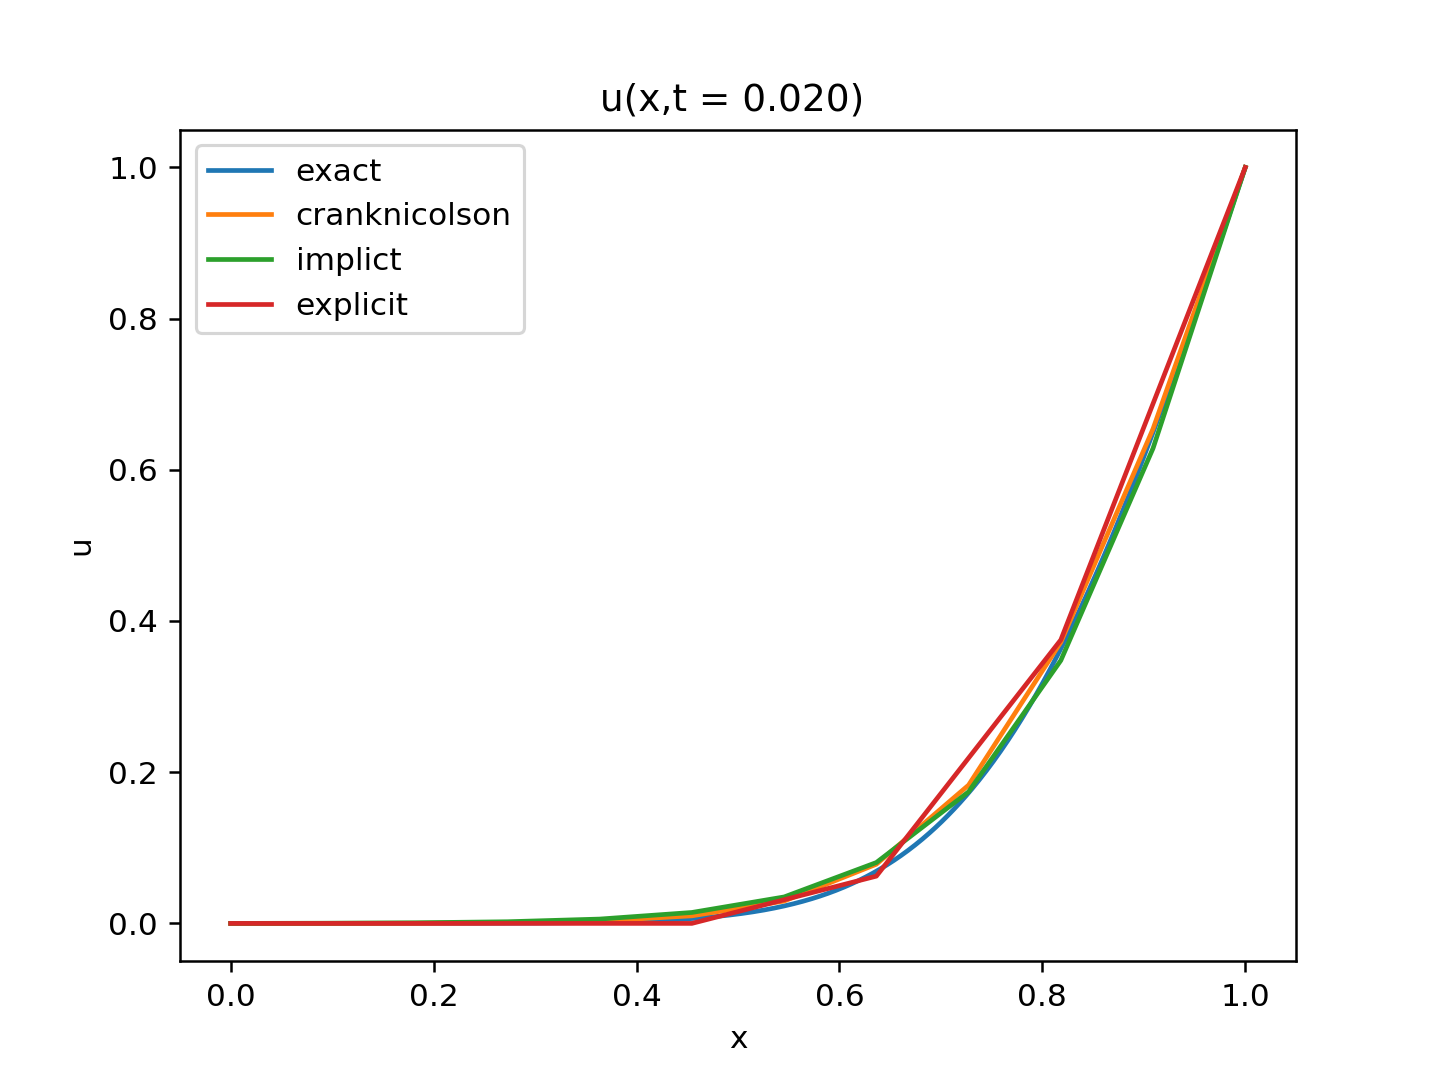
\includegraphics[width=\linewidth]{Nt200Nx10t02.png}
  \caption{The exact solution plotted together with the numerical ones $\alpha =1/2$. Nx = 10, Nt = 200. The solution of the explicit solver is still stable.}
  \label{fig:Nt200Nx10t02}
\end{figure} 


\begin{figure}
  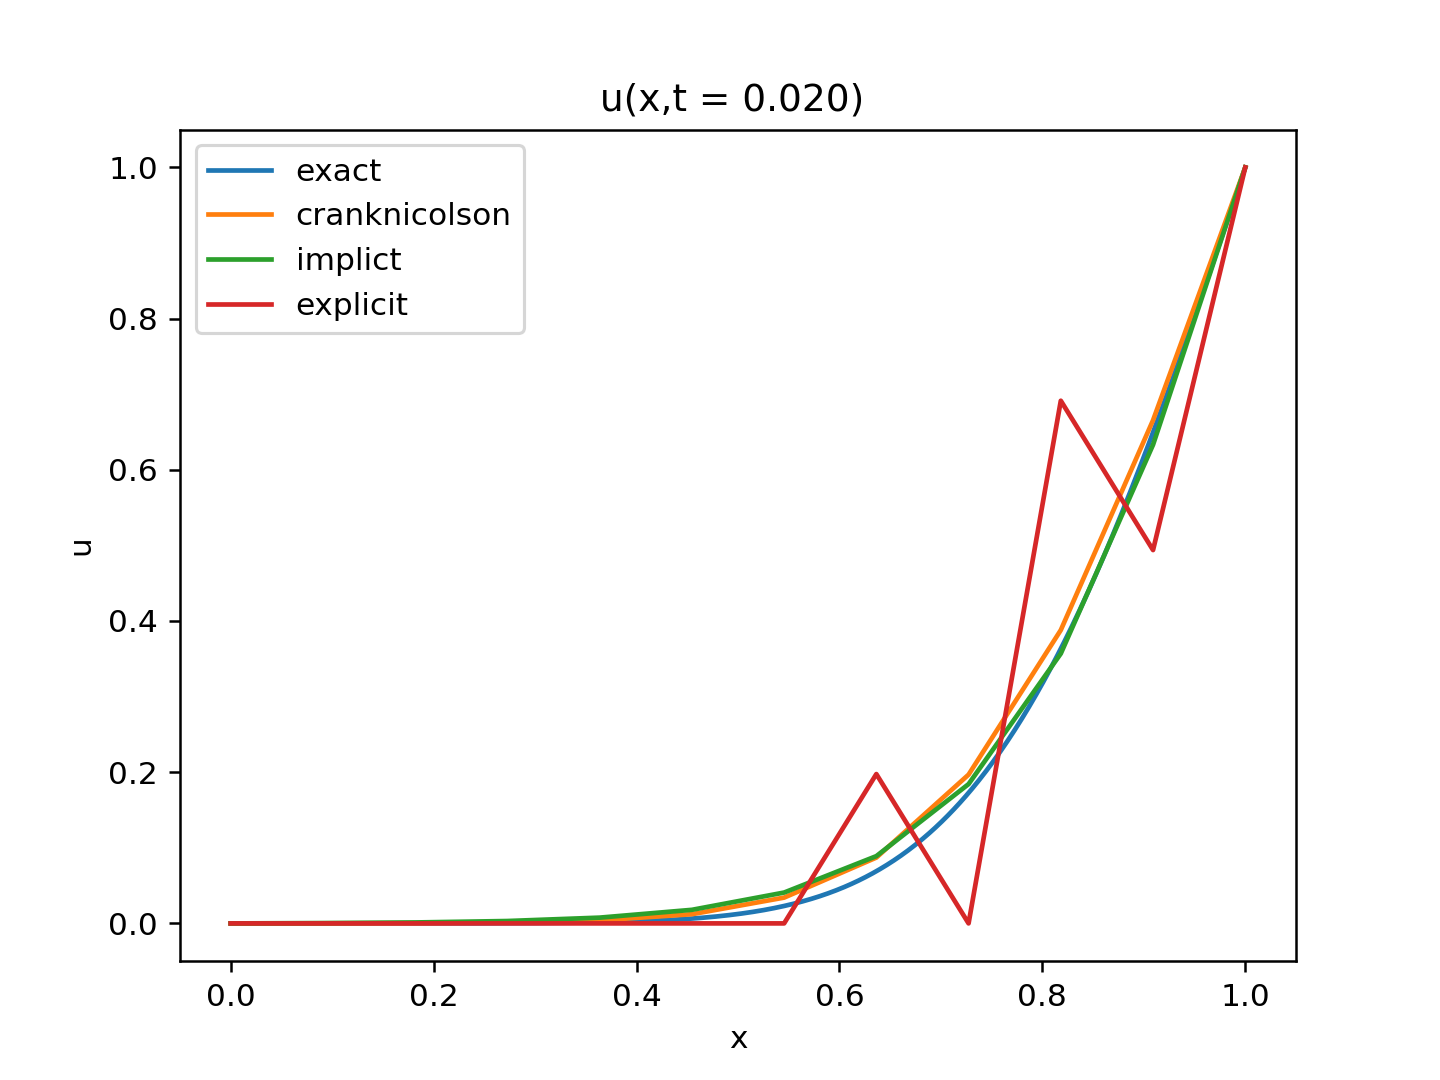
\includegraphics[width=\linewidth]{Nt150Nx10t02.png}
  \caption{The exact solution plotted together with the numerical ones $\alpha = 2/3$. Nx = 10, Nt = 150. The solution of the explicit solver has startet to go crazy.}
  \label{fig:Nt150Nx10t02}
\end{figure} 
The stability requirement of the explicit scheme is
$$\alpha =\frac{\Delta t}{(\Delta x)^2}= \frac{Nx^2}{Nt} <\frac{1}{2}$$
In figure \ref{fig:Nt200Nx10t02}, $\alpha = 1/2$, and the system is stable, also for the explicit solver. In figure \ref{fig:Nt150Nx10t02}, $\alpha = 2/3$, we see that the solutions from the Crank--Nicolson and the implicit solver are stable, while the solution of the explicit solver is not stable. I tried with even smaller Nt and kept Nx constant, and the smaller Nt got, the more bouncy was the solution. The explicit scheme was easy to implement, and it runs quickly for small \texttt{Nx}, but if you want high spatial resulution, you will soon discover the stability requirement is hard to meet, and that you are better off spending your time implementing the implicit scheme, rather than waiting for the explicit solver.
\subsection{The 2D diffusion equation}
\subsubsection{Homogenous boundaries}

\begin{figure}
  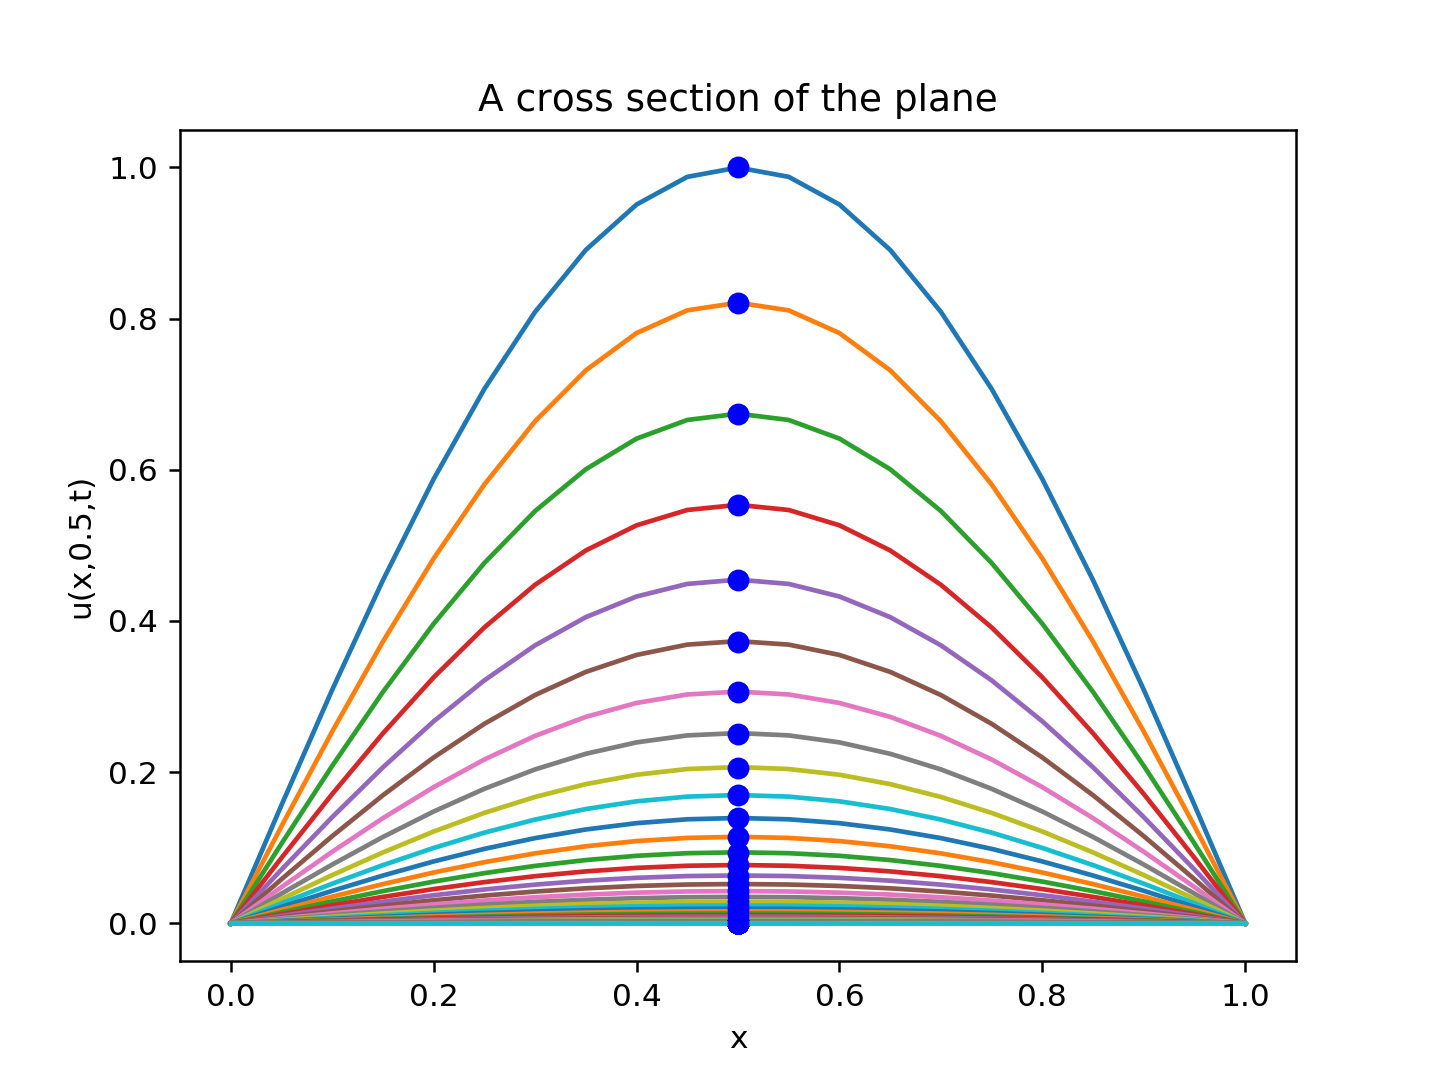
\includegraphics[width=\linewidth]{crosssection.png}
  \caption{A cross section parallell with the x axis. $u$ is plotted for $t \in [0,0.01, 0.02, ... , 1]$. Nx = Ny = 20, Nt = 100000. The solution has the shape of a sine curve. Blue dots are the theoretical values of $u(0.5,0.5,t)$.}
  \label{fig:crosssection}
\end{figure} 

\begin{figure}
  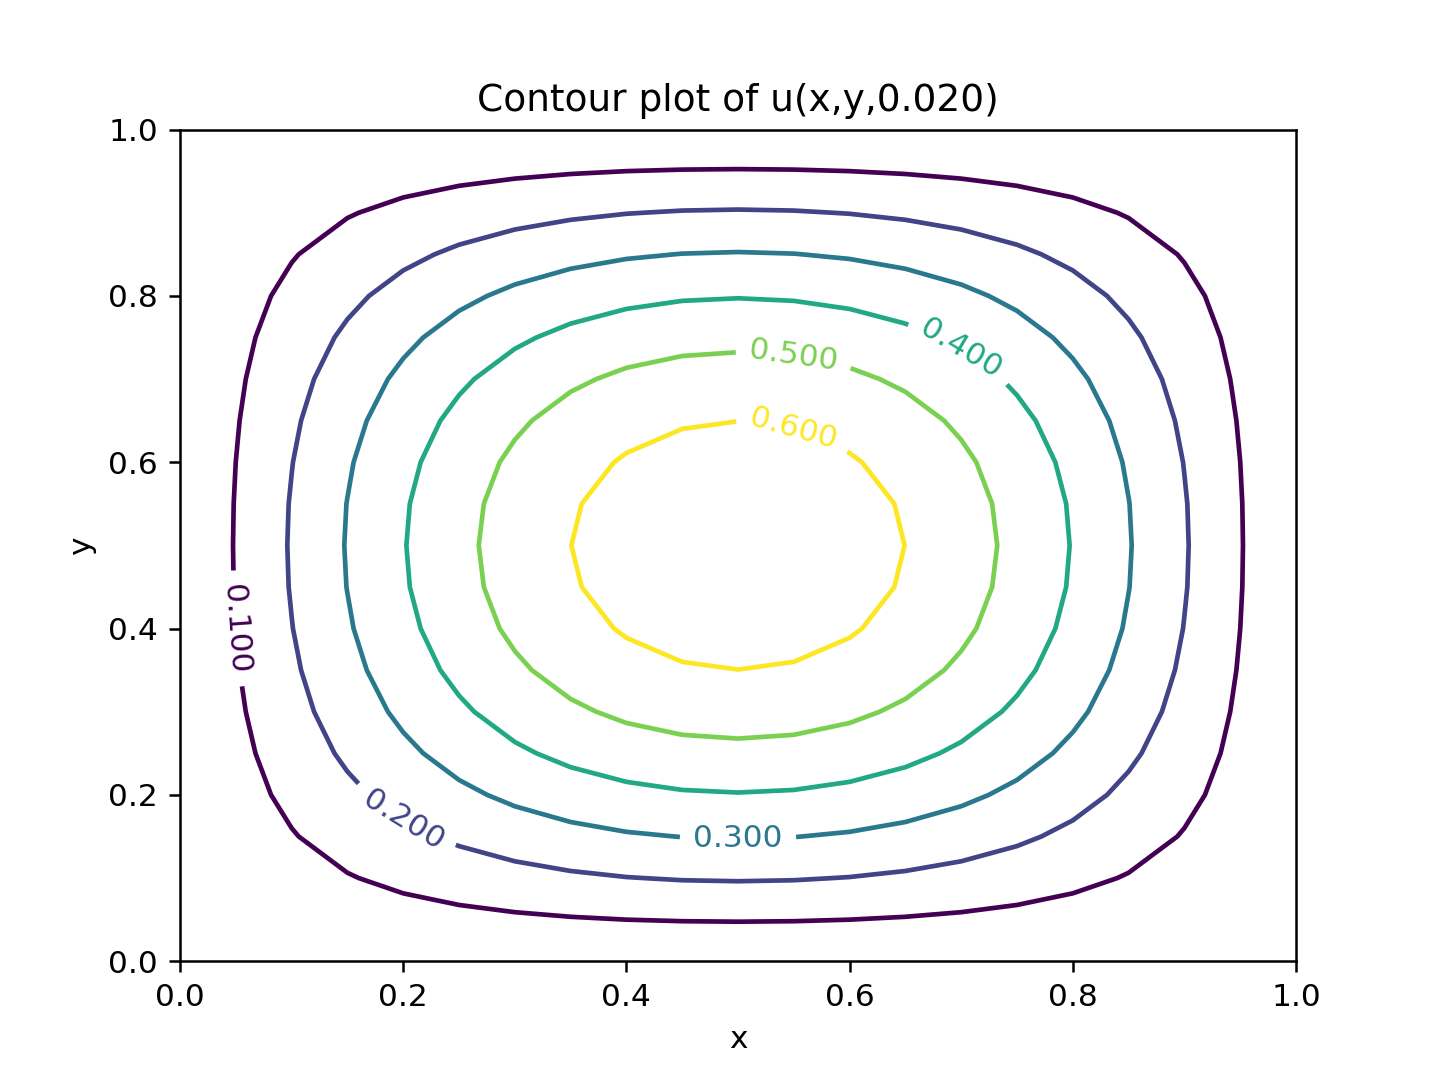
\includegraphics[width=\linewidth]{contoursine.png}
  \caption{A contour plot made at t=0.02. The curve has two mirror planes, $x=0.5$ and $y=0.5$. Nx =Ny = 20, Nt = 100000.}
  \label{fig:contoursine}
\end{figure} 
Because I found solving PDE's analytically rather tiresome, I chose the simplest initial and boundary conditions I could come up with. I am going to use the solution of section 3.2.1 to make sure that my 2D solver works as I expect. In order to see that the time dependency behaves as I expect, I plotted a cross section of the $xy$ plane, parallell to the $x$ axis. Figure \ref{fig:crosssection} shows that $u(x,0.5,t)$ has the shape of $\sin \pi x$, and that the amplitude gets smaller for larger $t$. $u$ is plotted for $t \in [0,0.01, 0.02, ... , 1]$.  According to the analytical solution, the amplitude should be $e^{-2\pi^2 t}$. For the first 10 solutions, the amplitudes are $$[  0.820,  0.673,  0.553,  0.454,
        0.372,  0.305,  0.251,  0.206,  0.169,  0.138]$$ The blue dots in figure \ref{fig:crosssection} are the analyticl values.  

Figure \ref{fig:contoursine} shows $u(x,y,0.02)$ which corresponds to the green line in \ref{fig:crosssection}. The curve has two mirror planes, $x=0.5$ and $y=0.5$. It has its highest point in the middle, and approaches zero in the edges. I feel confident that the numerical solution I find is the correct one, because it has the same behaviour as the analytical solution.
\subsubsection{Error and instability}
I did en attempt on error calculation. I had a small hope that calculating the local error of the first step (instead of the global error after many steps in time) would give errors that were more in agreement with the theoretical errors.  I used Nt= 10000 and Nx =10,20, 30, 40, and calculated the error of the very first solution, that is, at time $0.0001$. The expression I used for the error is $$\frac{||e^{-2\pi^20.0001}\sin\pi x-u_{numerical}||}{||e^{-2\pi^20.0001}\sin\pi x||}$$ The results were discouraging. 

Nx = 10 gave error
0.00194350451375

Nx = 20 gave error
0.00196775702548

Nx = 30 gave error
0.00197226135521

Nx = 40 gave error
0.00197383884111

In other words, the error did not change at all, even though the quality of the plots got better. It is clear that I have misunderstood something very important when it comes to error calculation, and because of the disappointment when it comes to the error's dependency on $\Delta x$, I did not feel the urge to go on and find the dependeny on $\Delta t$ .

With Nt= 10000, the system was stable for Nx = 50, but for Nx=60 it was absolutly out of control. Compared to the stability criterion of the 1D explicit scheme

$$\Delta t /(\Delta x)^2 = Nx^2/Nt = 60^2/10000 = 0.36<0.5$$
I can say that there must be a stronger stability criterion of the explicit shceme for the 2D problem. 

\begin{figure}[!tbp]
  \centering
  \begin{minipage}[b]{0.45\textwidth}
    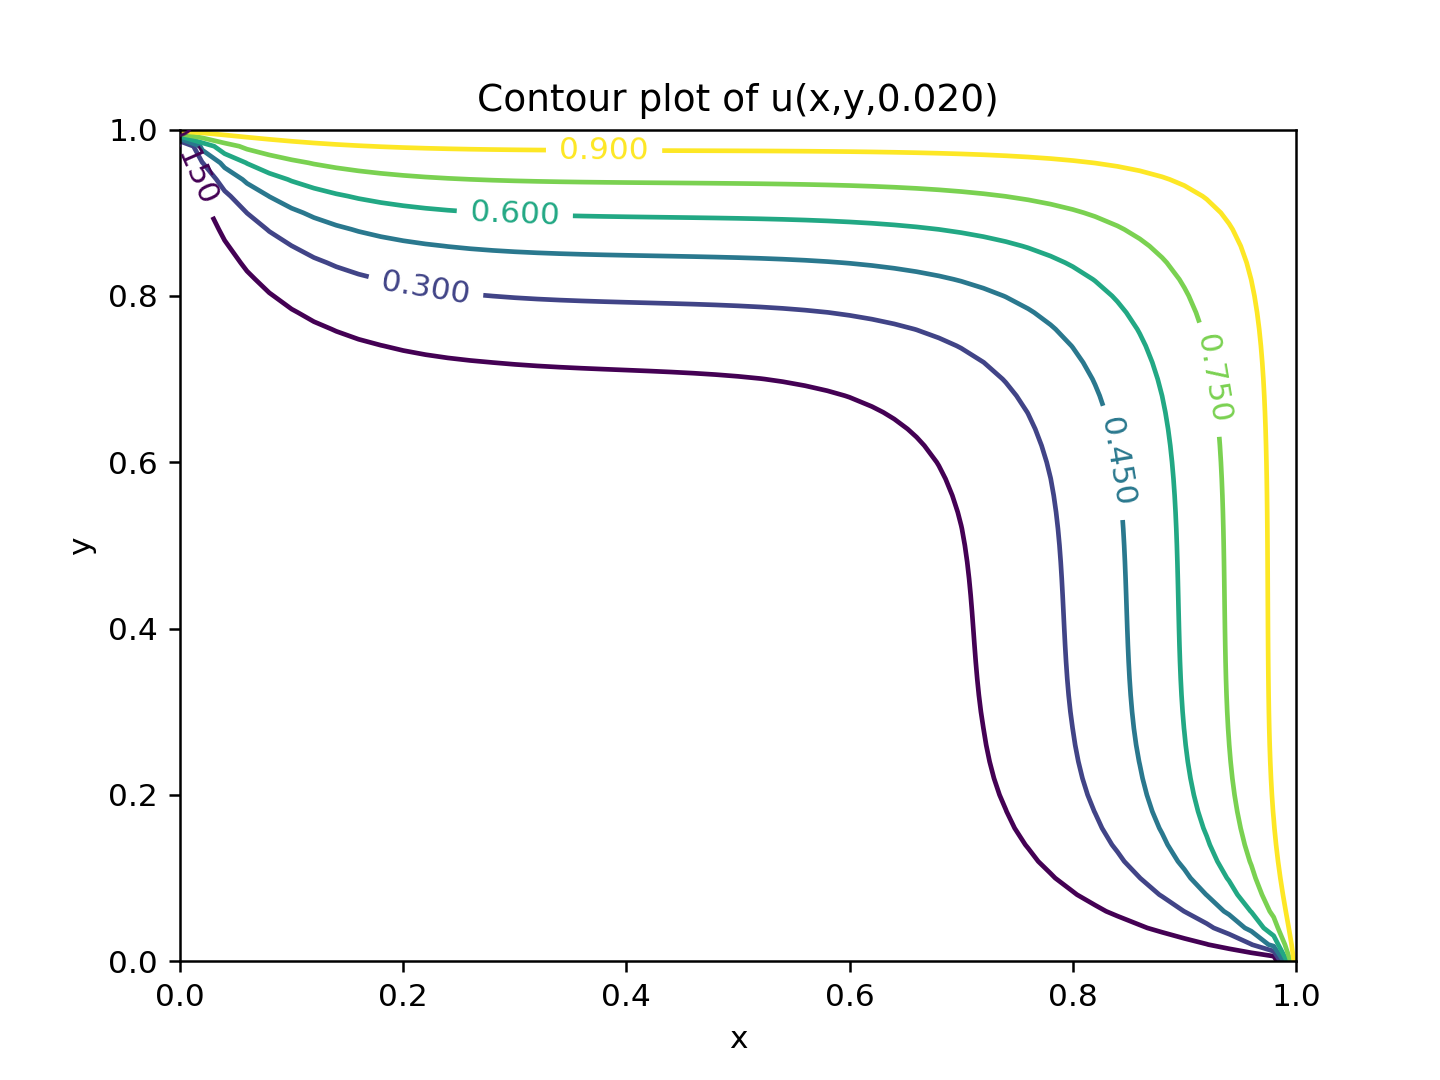
\includegraphics[width=\textwidth]{contour1.png}
  \end{minipage}
  \hfill
  \begin{minipage}[b]{0.45\textwidth}
    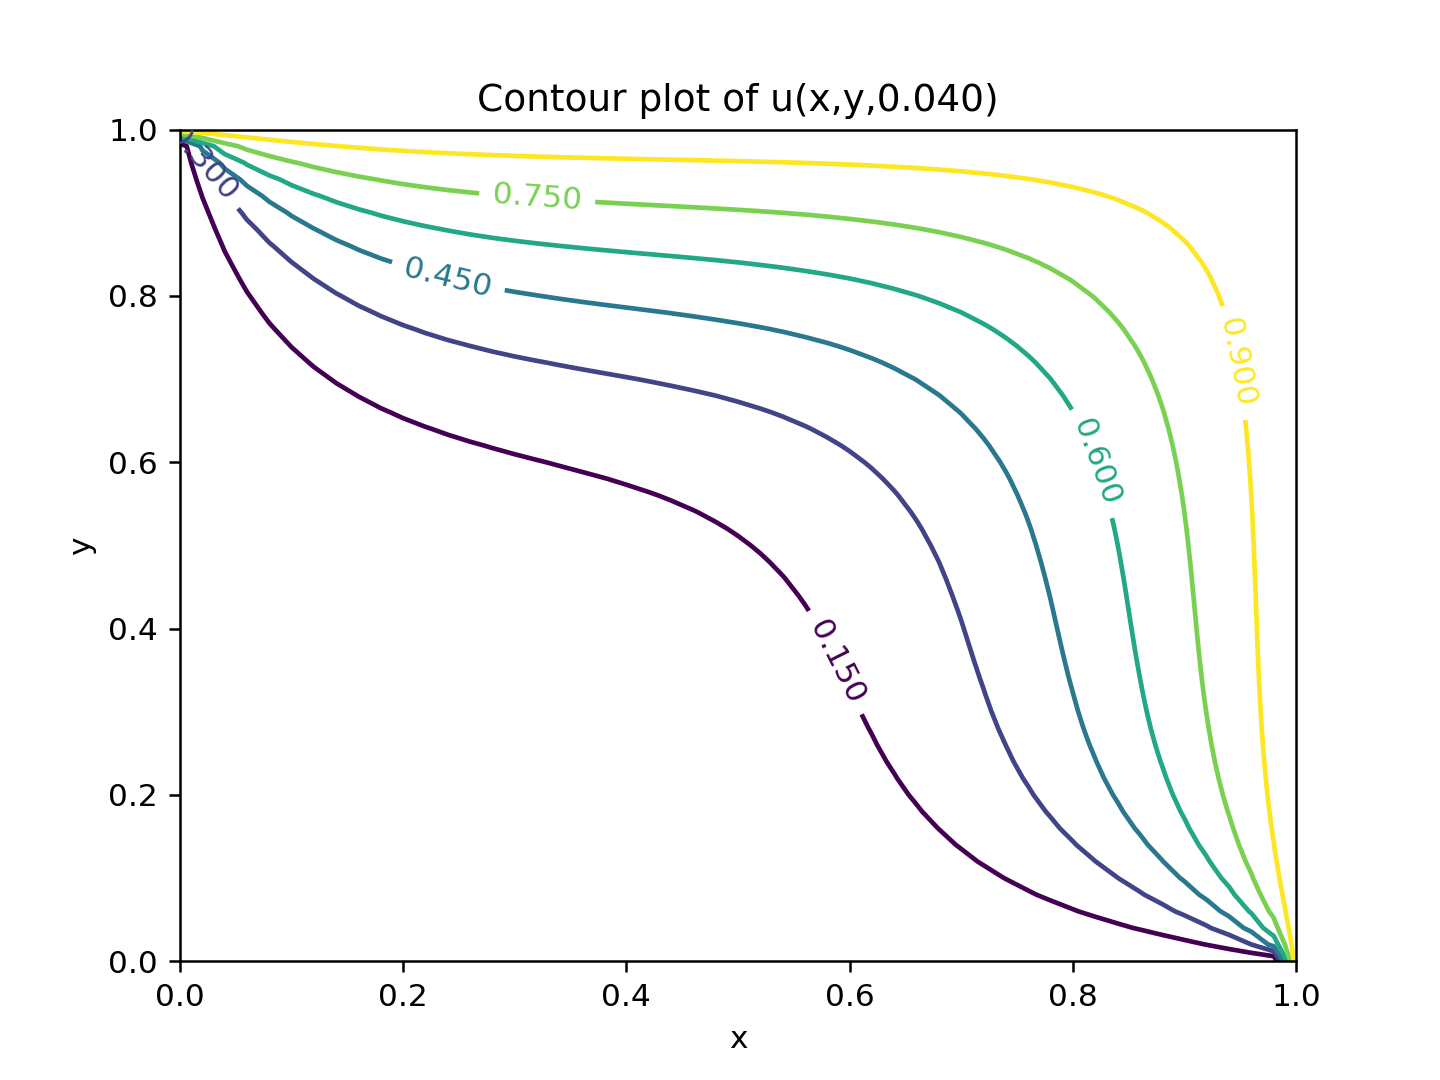
\includegraphics[width=\textwidth]{contour2.png}
  \end{minipage}
    \begin{minipage}[b]{0.45\textwidth}
    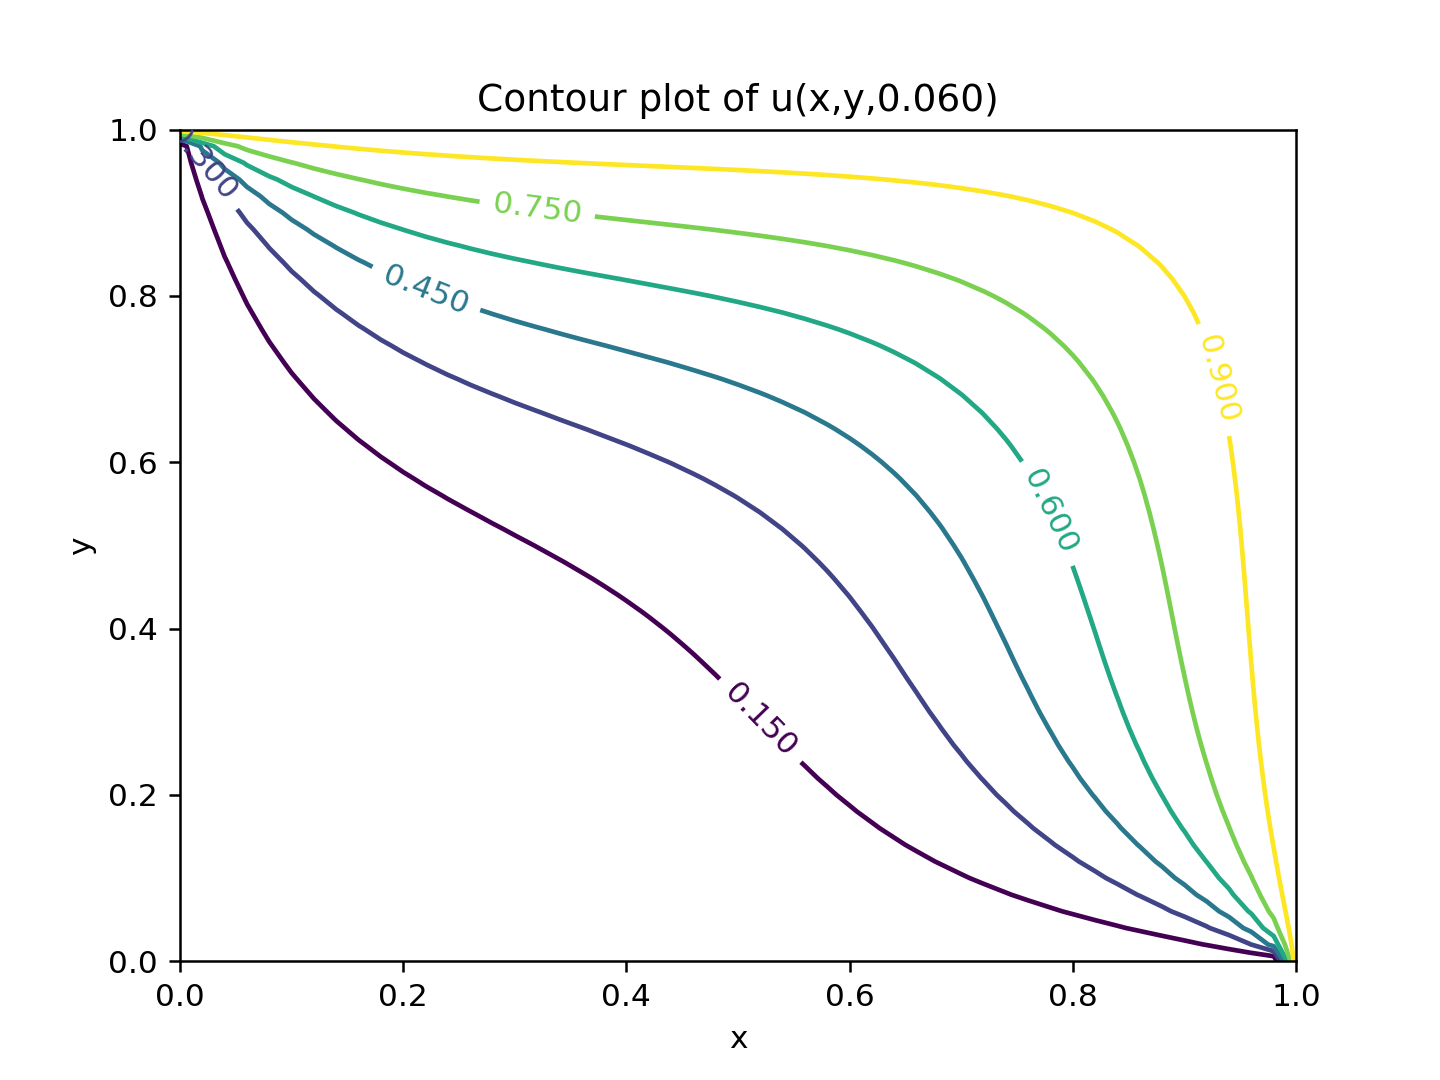
\includegraphics[width=\textwidth]{contour3.png}
  \end{minipage}
  \hfill
  \begin{minipage}[b]{0.45\textwidth}
    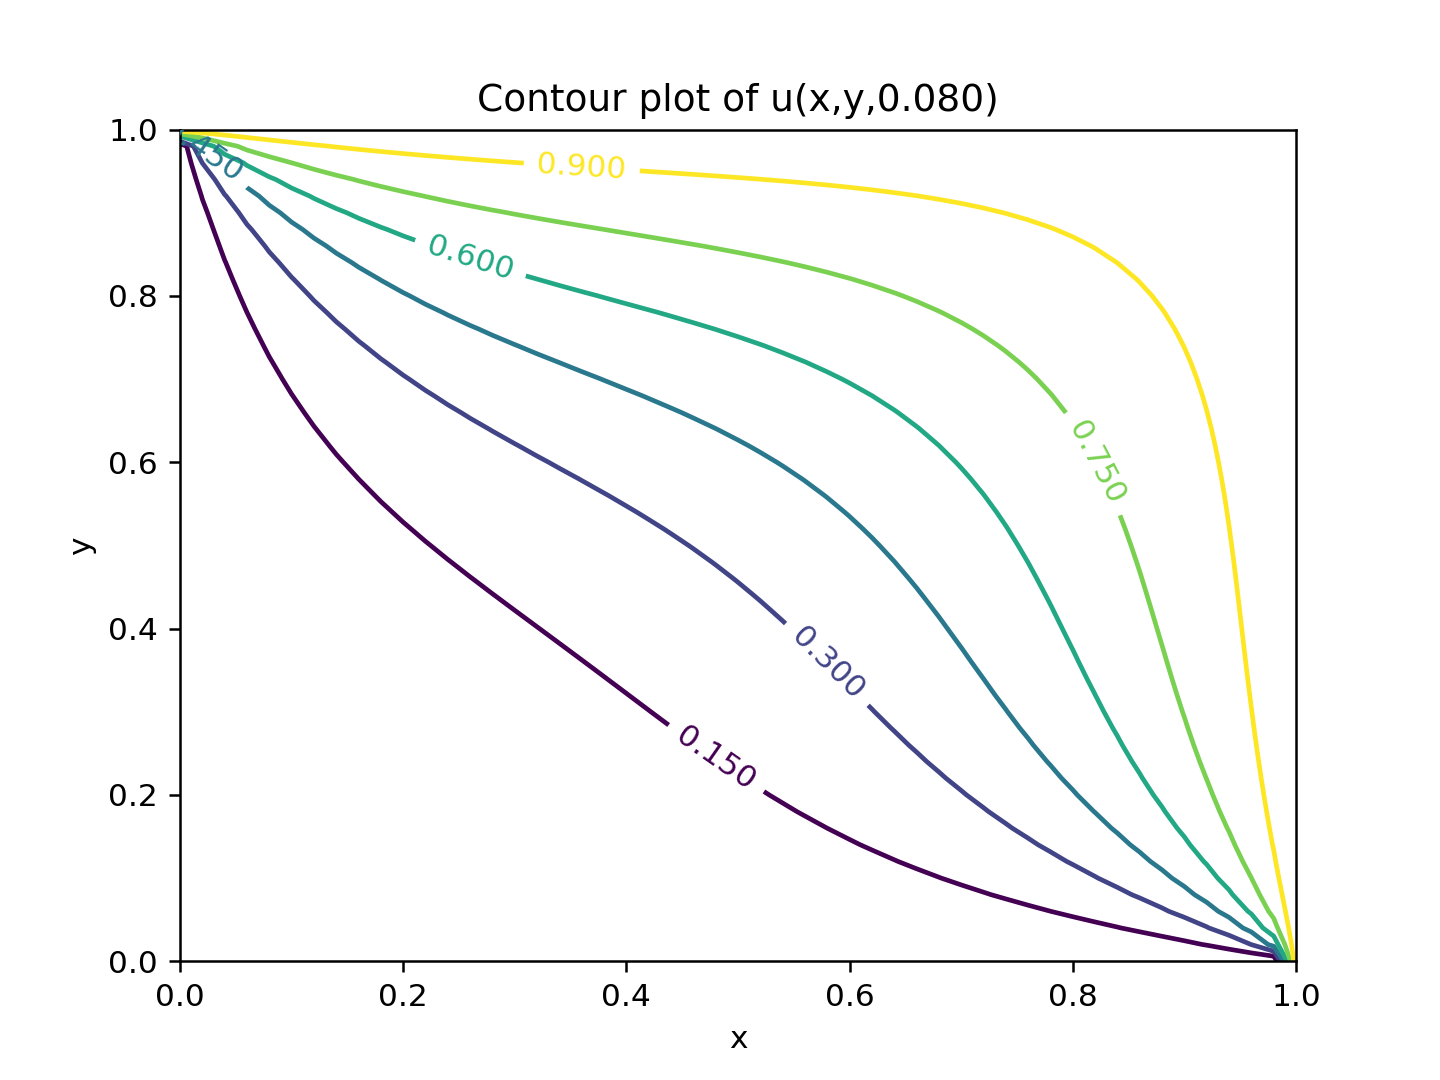
\includegraphics[width=\textwidth]{contour4.png}
  \end{minipage}
  \caption{The contour plots shows the development of u. u is plotted for $t=0.02,0.04,0.06, 0.08$.Nx = Ny = 50, Nt = 100000}
  \label{fig:contours}
\end{figure} 
\subsubsection{Nonhomogenous boundaries}
Even though I have a hard time evaluating the quality of my results, the solution I have found using my explicit solver resembles the analytical one. I am brave enough to think that the solver does its job, so I tried it on an other system, mentioned in section 3.2.2. The pysical problem in focus could be heat conduction in a block, where two sides of the block is in contact with a reservoir with high temperature, and the other two sides in contact with a reservoir of low temperature .Figure \ref{fig:contours} shows the progression of $u$ towards steady state. Figure \ref{fig:contour40} shows the system in equilibrium. The solution has two mirror planes, one along the $(0,0)(1,1)$ diagonal, and one along the $(0,1)(1,0)$ diagonal. The first reflects the symmetry of the boundary conditions, the other tells me that that I can switch the $x$ and $y$ values and still get the same result. In the corners, the plot of the soluton is not smooth. This is an artefact of the contour plot function in python. Instead of cutting off the contour lines at the point where no values are calculated, the contoul lines are all forced to continue to the edge of the plot. 
 \begin{figure}
  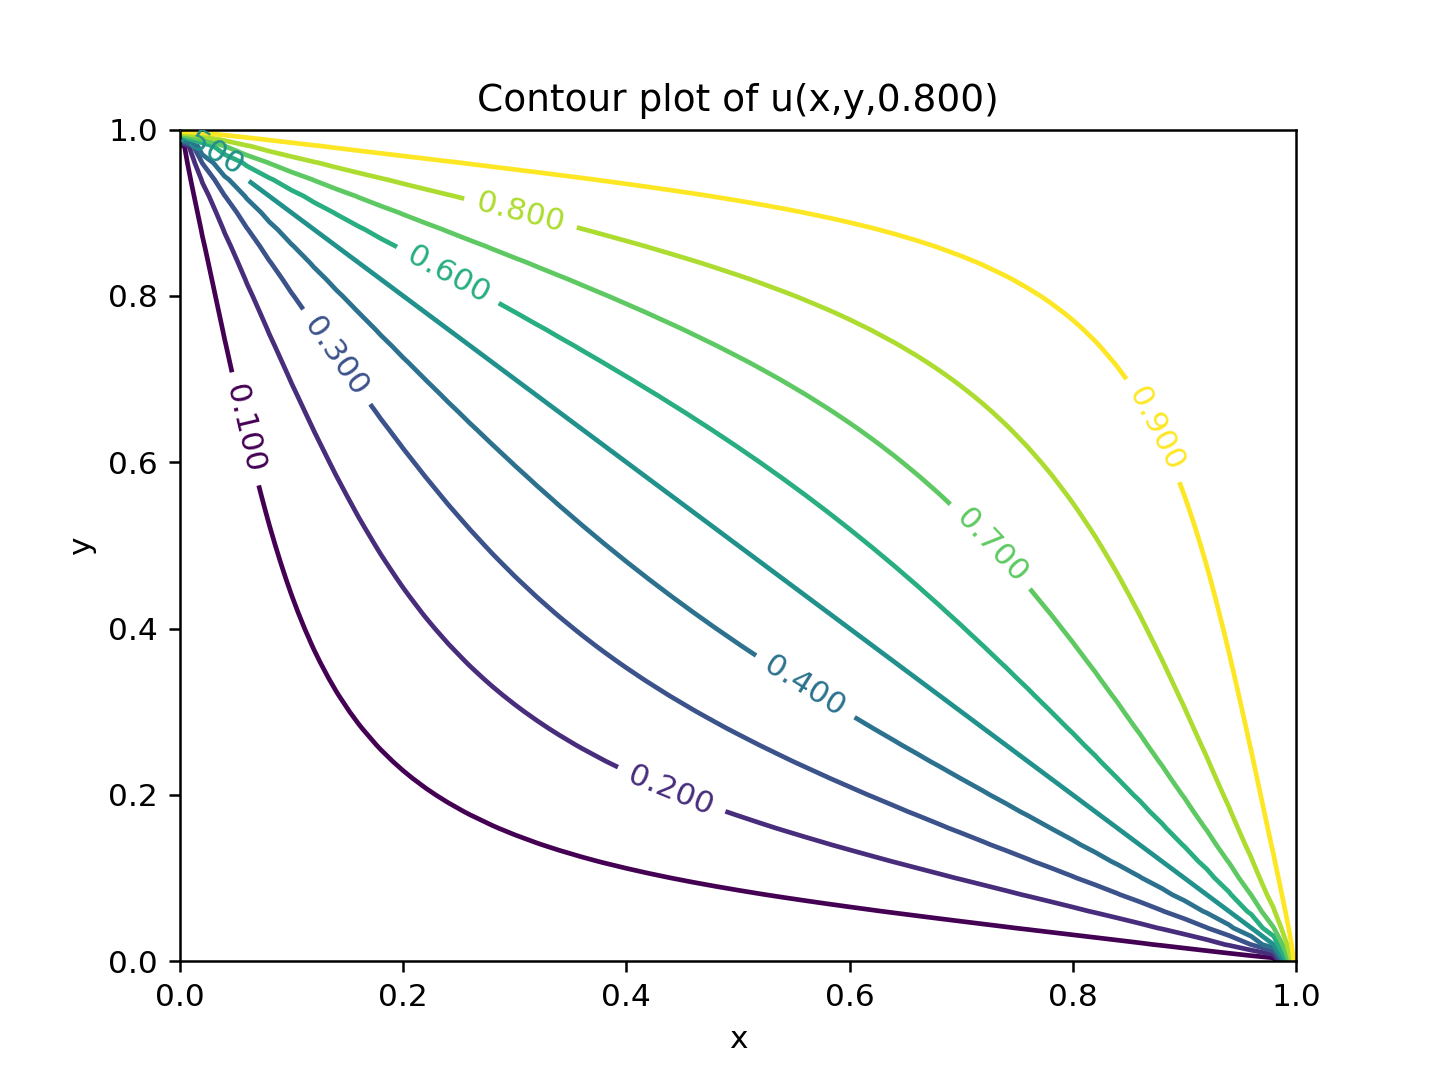
\includegraphics[width=\linewidth]{contour40.png}
  \caption{A contour plot made at t=0.8. Nx = Ny = 50, Nt = 100000. The system has reached equilibrium}
  \label{fig:contour40}
\end{figure} 
\section{Conclusion}
The explicit scheme, the implicit scheme and the Cranck--Nicolson scheme gave the same quality of the solution as long as the stability requirement of the explicit scheme were met. For high spatial resolution, the explicit scheme require incredibly many time steps, which makes it unsuitable for problems where the quality of the solution is important. The implicit scheme does not have stability requirements, but is still quite easy to implement, as is is the solution of a matrix equation with a tridiagonal matrix. My implementation of the Crank--Nicolson scheme did not prove to have smaller error than the others, for ths reason I would prefer the implicit scheme. The fact that the error did not behave as expected -- it did not decrease with smaller time steps, is a serous flaw of my project, and it is something I definitely have to investigate further, because I need to be able to make reliable error analysis in the future e.g.  in my masters thesis.

For two dimensions, I have only implemented the explicit scheme. It made me capable of finding solutions of the 2D diffusion equation that are boring or difficult to find analytically. Furter work with the diffusion equation would involve the implementation of the 2D implicit scheme, to get high resolution without extremely many time steps. 

\begin{thebibliography}{1}

\bibitem{PDE}
M. Hjort-Jensen: Computational Physics: Partial Differential Equations,
\\\texttt{http://compphysics.github.io/ComputationalPhysics/doc/pub/pde/pdf/pde-print.pdf}

\bibitem{Boyce}
R. C. DiPrima and W. E. Boyce: Elementary Differential Equations and Boundary Value Problems,
\\\texttt{http://www.labma.ufrj.br/~mcabral/cursos/2017-1/Boyce-cap10.5.pdf}

\bibitem{Project1} 
S. Videm: Computational Physics: Project 1,
\\\texttt{https://github.com/sigrivi/Project1}





\end{thebibliography}
\end{document}